\documentclass[12pt]{article}

\usepackage{amssymb,amsmath,amsthm}
\usepackage{bm}
\usepackage{mathtools}
\usepackage{physics}% for a "straight" differential

\newcommand{\R}{\mathbb{R}}
\newcommand{\C}{\mathbb{C}}
\newcommand{\Z}{\mathbb{Z}}
\newcommand{\Q}{\mathbb{Q}}
\newcommand{\N}{\mathbb{N}}
\newcommand{\F}{\mathbb{F}}
\newcommand{\E}{\mathbb{E}}
\newcommand{\Pbb}{\mathbb{P}}
\newcommand{\calP}{\mathcal{P}}

\newcommand{\parallelsum}{\mathbin{\!/\mkern-5mu/\!}}

\newcommand\Myperm[2][^n]{\prescript{#1\mkern-2.5mu}{}P_{#2}}
\newcommand\Mycomb[2][^n]{\prescript{#1\mkern-0.5mu}{}C_{#2}}

\newcommand{\diff}{\text{d}}
\newcommand{\Diff}{\text{D}}

\newcommand{\vN}{\mathbf{N}}
\newcommand{\vn}{\mathbf{n}}
\newcommand{\ve}{\mathbf{e}}
\newcommand{\vv}{\mathbf{v}}
\newcommand{\vx}{\mathbf{x}}

\newcommand{\la}{\langle}
\newcommand{\ra}{\rangle}

\usepackage[margin=1.25in]{geometry}
\usepackage{fancyhdr}
\usepackage{setspace}
\pagestyle{fancy}
\usepackage{amsfonts}

\usepackage{graphicx} 
\usepackage{float} 
\usepackage{subfigure} 

\newtheorem{theorem}{Theorem}
\newtheorem*{theorem*}{Theorem}
\newtheorem{lemma}[theorem]{Lemma}
\newtheorem*{lemma*}{Lemma}
\newtheorem{sublemma}{Lemma}[section]
\newtheorem*{sublemma*}{Lemma}

\title{Homework}
\lhead{MATH 4302}
\chead{Assignment 2}
\rhead{Qu Tianyong, 3035770721}

\linespread{1.2}
\begin{document}
	
%	\begin{figure}[H] 
%		\centering 
%		\includegraphics[width=xx\textwidth]{xx} 
%		\caption{xx} 
%		\label{xx} 
%	\end{figure}

%	\Myperm{k} = \frac{n!}{(n-k)!}\quad
%	\Mycomb{k} = \frac{n!}{k!(n-k)!}\quad
%	\Myperm[m]{k} = \frac{m!}{(m-k)!}\quad
%	\Mycomb[m]{k} = \frac{m!}{k!(m-k)!}\quad

%$$=\left\{
%	\begin{array}{rcl}
%	\end{array}
%\right.$$


\begin{enumerate}
	%1
	\item[1.]
	\begin{enumerate}
		%a
		\item[(1)]
		\begin{proof}
		    By the fundamental theorem of algebra, the irreducible elements in $R$\ are polynomials of degree one. So we assume that $f=ax+b$, where $a,b\in\C$\ and $a$\ is nonzero. Now for any $g\in R$, note that $R$\ is an Euclidean domain, we can write $g=f\cdot h+r$, where $h,r\in R$\ and $\deg(r)<\deg(f)$. Since $\deg(f)=1$, $r$\ is a constant. Thus we have $R/\la f\ra$\ is a subfield of $\C$. Consider the set $\{ax+c:c\in C\}$. The projection of this set under $f$\ is exactly the set $\C$. Therefore we have $R/\la f\ra=\C$.
		\end{proof}
		%b
		\item[(2)]
		\begin{proof}
		    By the fundamental theorem of algebra, $f$\ is of degree one or of degree two and has delta $\Delta<0$.\par
		    \quad Case 1: $f=ax+b$, where $a,b\in\R$\ and $a$\ is nonzero. Consider the set $\{ax+c:c\in\R\}\subset R$, the projection of this set under $f$\ is exactly the set $\R$. So $\R$\ is a subfield of a field isomorphic to $R/\la f\ra$. Note that $R$\ is a Euclidean domain, so every $g\in R$\ can be written as $g=f\cdot h+r$, where $h,r\in R$\ and $\deg(r)<\deg(f)=1$. Thus $\deg(r)=0$, $r$\ is a constant. Therefore $R/\la f\ra\cong\R$.\par
		    \quad Case 2: $f=ax^2+bx+c$, where $a,b,c\in\R$, $a$\ is nonzero and $\Delta=b^2-4ac<0$. Since $R$\ is a Euclidean domain, any $g\in R$\ can be written as $g=f\cdot h+r$, where $h,r\in R$\ and $\deg(r)<\deg(f)=2$. So $r$\ has degree one or two. Thus $R/\la f\ra$\ is isomorphic to a subfield of $\C$. And the set $\{ax^+bx+d:d\in\R\}$\ and the set $\{ax^2+ex+c:e\in\R\}$\ shows that $R/\la f\ra$\ is isomorphic to $\C$\ itself. Therefore either $R/\la f\ra\cong\R$\ or $R/\la f\ra\cong\C$.
		\end{proof}
	\end{enumerate}
	%2
	\item[2.]
	\begin{enumerate}
		%a
		\item[(1)]
		\begin{proof}
		    Assume to the contrary that $f$\ is reducible. Then $f$\ has a linear factor since $f$\ is a cubic function. However $f(0)=f(1)=f(2)=1$, which means $f$\ does not have linear factor. Thus $f$\ is irreducible. This field has $3^3=27$\ elements.
		\end{proof}
		%b
		\item[(2)]
		\textit{Solution.}
		\begin{figure}[H] 
		    \centering 
		    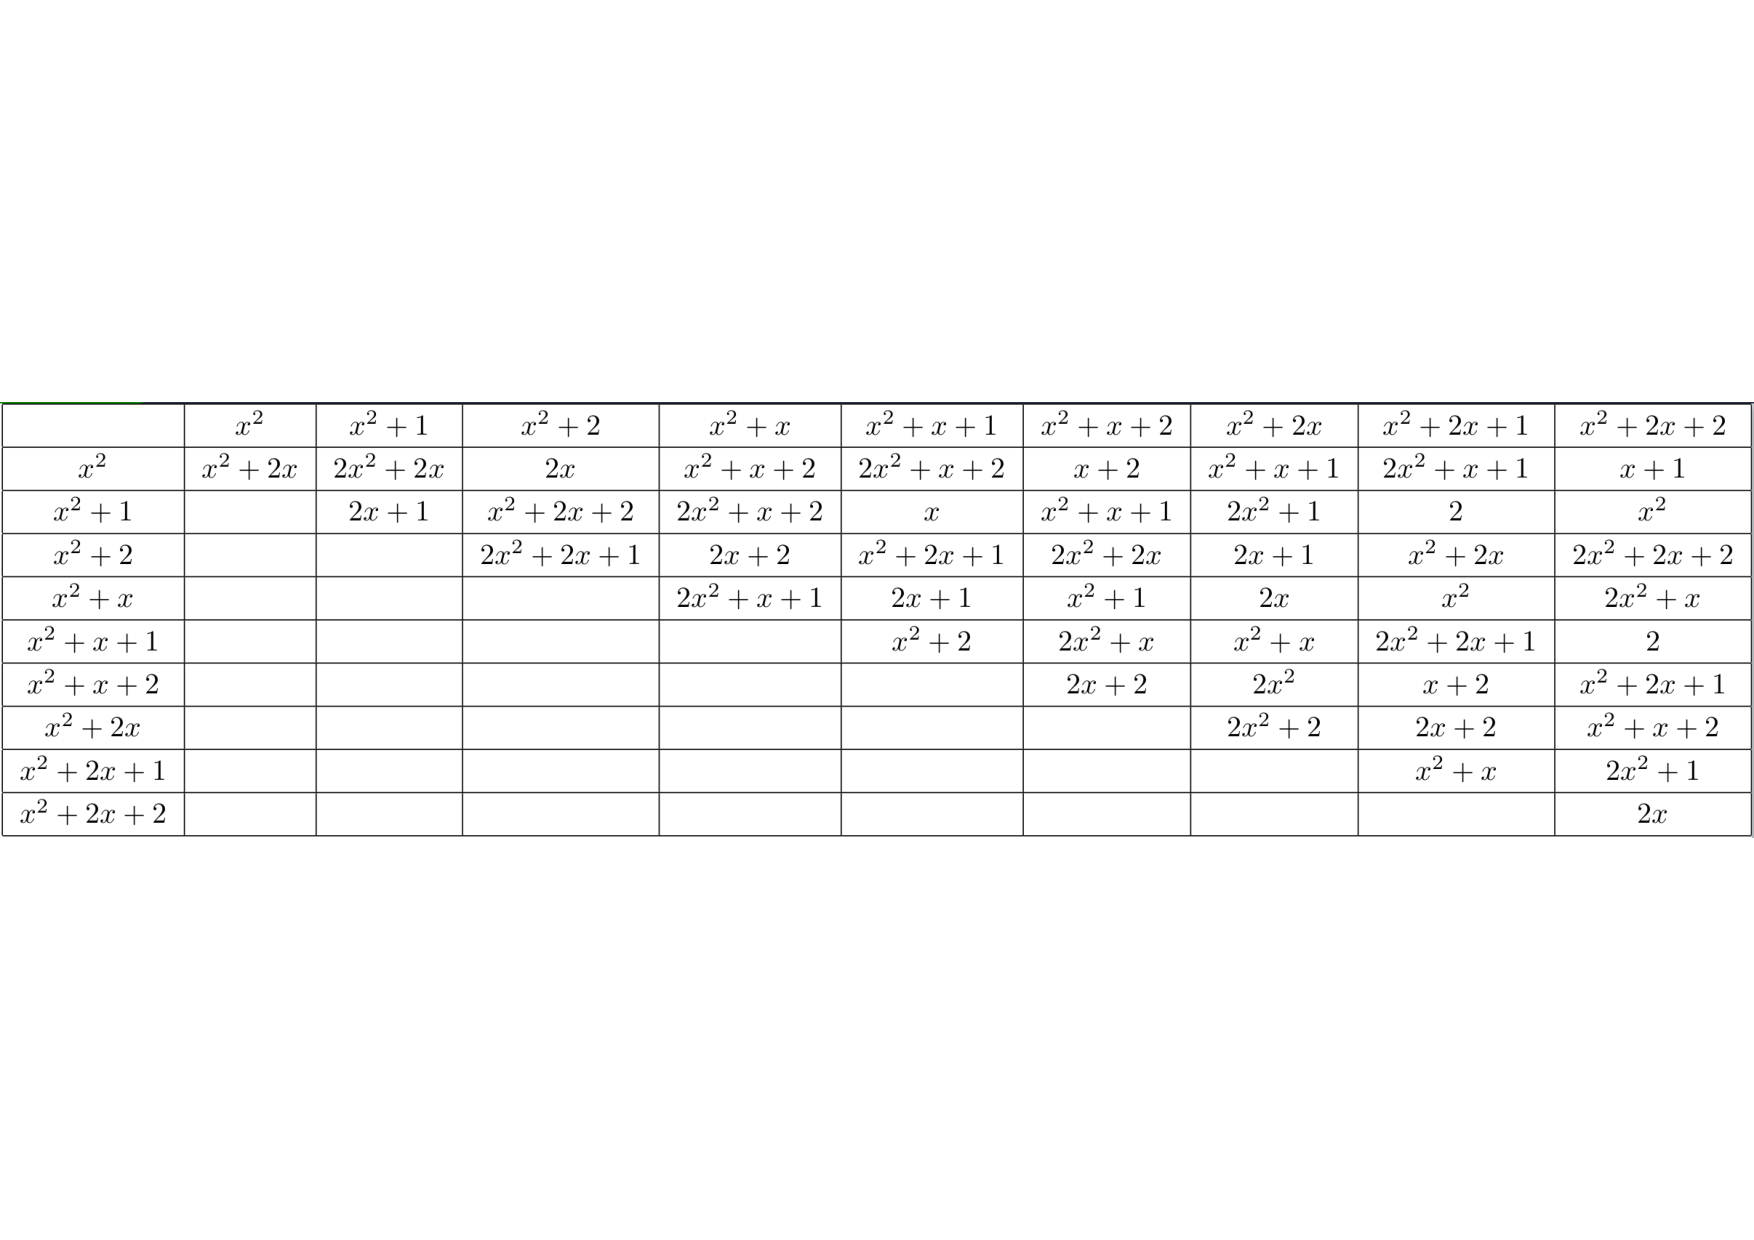
\includegraphics[width=1.1\textwidth]{table} 
%		    \caption{xx} 
%	    	\label{xx} 
    	\end{figure}
	\end{enumerate}
%\begin{tabular}{|c|c|c|c|c|c|c|c|c|c|}
%	    \hline
%        &$x^2$&$x^2+1$&$x^2+2$&$x^2+x$&$x^2+x+1$&$x^2+x+2$&$x^2+2x$&$x^2+2x+1$&$x^2+2x+2$\\
%        \hline
%        $x^2$&$x^2+2x$&$2x^2+2x$&$2x$&$x^2+x+2$&$2x^2+x+2$&$x+2$&$x^2+x+1$&$2x^2+x+1$&$x+1$\\
%        \hline
%        $x^2+1$&&$2x+1$&$x^2+2x+2$&$2x^2+x+2$&$x$&$x^2+x+1$&$2x^2+1$&$2$&$x^2$\\
%        \hline
%        $x^2+2$&&&$2x^2+2x+1$&$2x+2$&$x^2+2x+1$&$2x^2+2x$&$2x+1$&$x^2+2x$&$2x^2+2x+2$\\
%        \hline
%        $x^2+x$&&&&$2x^2+x+1$&$2x+1$&$x^2+1$&$2x$&$x^2$&$2x^2+x$\\
%        \hline
%        $x^2+x+1$&&&&&$x^2+2$&$2x^2+x$&$x^2+x$&$2x^2+2x+1$&$2$\\
%        \hline
%        $x^2+x+2$&&&&&&$2x+2$&$2x^2$&$x+2$&$x^2+2x+1$\\
%        \hline
%        $x^2+2x$&&&&&&&$2x^2+2$&$2x+2$&$x^2+x+2$\\
%        \hline
%        $x^2+2x+1$&&&&&&&&$x^2+x$&$2x^2+1$\\
%        \hline
%.       $x^2+2x+2$&&&&&&&&&$2x$\\
%        \hline
%\end{tabular}
	%3
	\item[3.]
	\begin{enumerate}
		%a
		\item[(1)]
		\textit{Solution.}
		    $f$\ is irreducible over $\Q$. By Eisenstein's Criteria, $3|a_0,a_1,\ldots,a_8$, but $3\nmid a_9$\ and $9\nmid a_0$.
		%b
		\item[(2)]
		\textit{Solution.}
		    $f$\ is irreducible over $\Q$. Take $p=2$, note that $\pi_2(f)=x^4+x+1$\ has no root over $Z_2[x]$, thus it has no proper factorization over $\Z[x]$, and therefore is irreducible over $\Q[x]$.
		%c
		\item[(3)]
		\textit{Solution.}
		    $f$\ is irreducible over $\Q$. Take $p=3$, note that $\pi_2(f)=x^4+x^3+2x+1$\ has no root over $Z_3[x]$\ ($\pi_2(f)(0)=1$,$\pi_2(f)(1)=2$,$\pi_2(f)(2)=2$), thus it has no proper factorization over $\Z[x]$, and therefore is irreducible over $\Q[x]$.
	\end{enumerate}
	%4
	\item[4.]
	\begin{enumerate}
		%a
		\item[(1)]
		\begin{proof}
		    For any $a\in\Z$, $f=x-a\in\Z[x]$\ is a monic polynomial such that $a$\ is its root, so $\Z\subset\Q\cap\bar{\Z}$. If a rational number $\frac{b}{a}$\ is in $\bar{\Z}$\ where $\gcd(a,b)=1$\ and $a\neq1$, assume that $f=x^n+a_{n-1}x^{n-1}+\cdots+a_1x+a_0$\ is a monic function which has $\frac{b}{a}$\ as its root. Then
		    $$f(\frac{b}{a})=\frac{b^n}{a^n}+a_{n-1}\frac{b^{n-1}}{a^{n-1}}+\cdots+a_1\frac{b}{a}+a_0=0,$$
		    $$b^n+a_{n-1}b^{n-1}a+\cdots+a_1ba^{n-1}+a_0a^n=0.$$
		    So $a|b^n=-a_{n-1}b^{n-1}a+\cdots+a_1ba^{n-1}+a_0a^n$, contradicts the assumption that $\gcd(a,b)=1$.\par
		    \quad Recall that the intersection of two field is again a field, we deduce that $\bar{\Z}$\ is not a field since $\Z$\ is not a field.
		\end{proof}
		%b
		\item[(2)]
		\begin{enumerate}
		    \item[(a)]
		    \textit{Solution.}
                $$R(f,g)=\det
                \begin{bmatrix}
                    2&2&1&0\\
                    0&2&2&1\\
                    -2&0&1&0\\
                    0&-2&0&1
                \end{bmatrix}
                =8.$$
		    \item[(b)]
		    \textit{Solution.}
                $$R(f,g)=\det
                \begin{bmatrix}
                    b&a&1\\
                    a&2&0\\
                    0&a&2
                \end{bmatrix}
                =4b-a^2.$$
		    \item[(c)]
		    \textit{Solution.}
                $$R(f,g)=\det
                \begin{bmatrix}
                    b&a&0&1&0\\
                    0&b&a&0&1\\
                    a&0&3&0&0\\
                    0&a&0&3&0\\
                    0&0&a&0&3
                \end{bmatrix}
                =27b^2+4a^3.$$
		\end{enumerate}
		%c
		\item[(3)]
		\begin{proof}
		    Since $f(x)$\ has a root $\alpha$\ and $g(z-x)$\ has a root $z-\beta$, the resultant has $\alpha-(z-\beta)=\alpha+\beta-z$\ as its factor. Therefore $P(z)$\ has a root $\alpha+\beta$.\par
		    \quad Since $f(x)$\ has a root $\alpha$\ and $x^ng(\frac{z}{x})$\ has a root $\frac{z}{\beta}$, the resultant has $\alpha-\frac{z}{\beta}=\beta(\alpha\beta-z)$\ as its factor. Therefore $Q(z)$\ has a root $\alpha\beta$. Here we multiply $x^n$\ in front of $g(\frac{z}{x})$\ in order to make $Q(z)$\ monic.
		\end{proof}
		\begin{enumerate}
		    \item[(a)]
		    \textit{Solution.}
	            $f(x)=x^2+2x+2$\ has $\alpha=1+i$\ as its root and $g(x)=x^2-2$\ has $\beta=\sqrt{2}$\ as its root. Therefore
	            $$P(z)=z^4-4z^3+4z^2+8,$$
	            $$Q(z)=z^4+16.$$
            \item[(b)]
            \textit{Solution.}
                $f(x)=x^2-2$\ has $\alpha=\sqrt{2}$\ as its root and $g(x)=x^2+3$\ has $\beta=i\sqrt{2}$\ as its root. Therefore
	            $$P(z)=z^4+2z^2+25,$$
	            $$Q(z)=z^2+6.$$
		\end{enumerate}
	\end{enumerate}
\end{enumerate}

\end{document}